\maketitle

\section{Introduction}

\begin{frame}[fragile]{Motivation}
\centering
\only<1>{
\includegraphics[width=\textwidth]{img/compiler_complaint.png}}

\only<2>{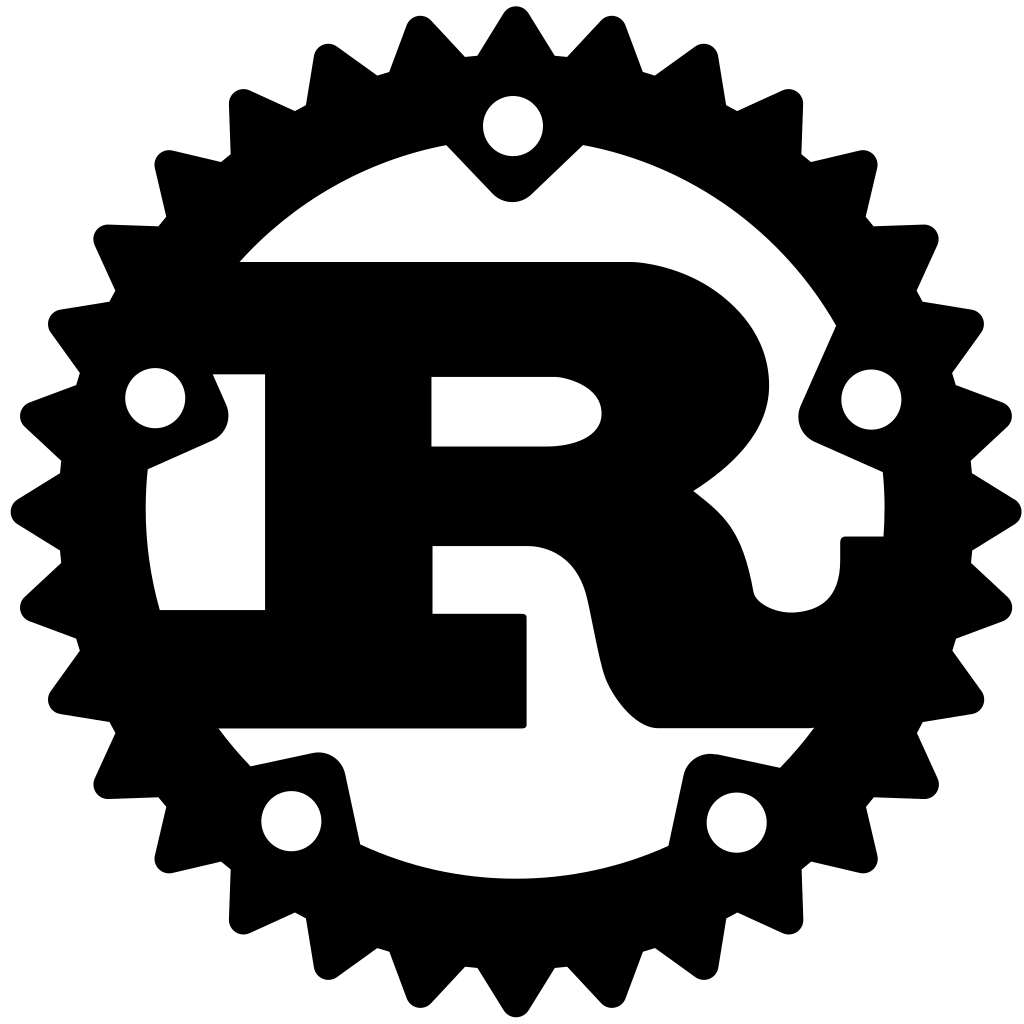
\includegraphics[width=0.3\textwidth]{img/rust.png}}

\begin{onlyenv}<3>
\begin{lstlisting}[style=short, language=Rust]
/// Returns the square of `x`. Squares are non-negative.
fn square(x: i32) -> i32 { -2 * x }
\end{lstlisting}
\end{onlyenv}

\begin{onlyenv}<4>
\begin{lstlisting}[style=short, language=Rust]
/// Returns the square of `x`. Squares are non-negative.
#[post(ret >= 0)]
fn square(x: i32) -> i32 { -2 * x }
// postcondition INVALID
\end{lstlisting}
\end{onlyenv}
\end{frame}


\begin{frame}{Presenting our tool}
  \begin{columns}
  \column{0.5\textwidth}
  \centering
  \Large{\texttt{rust-stainless}}

  \column{0.5\textwidth}
  \centering
  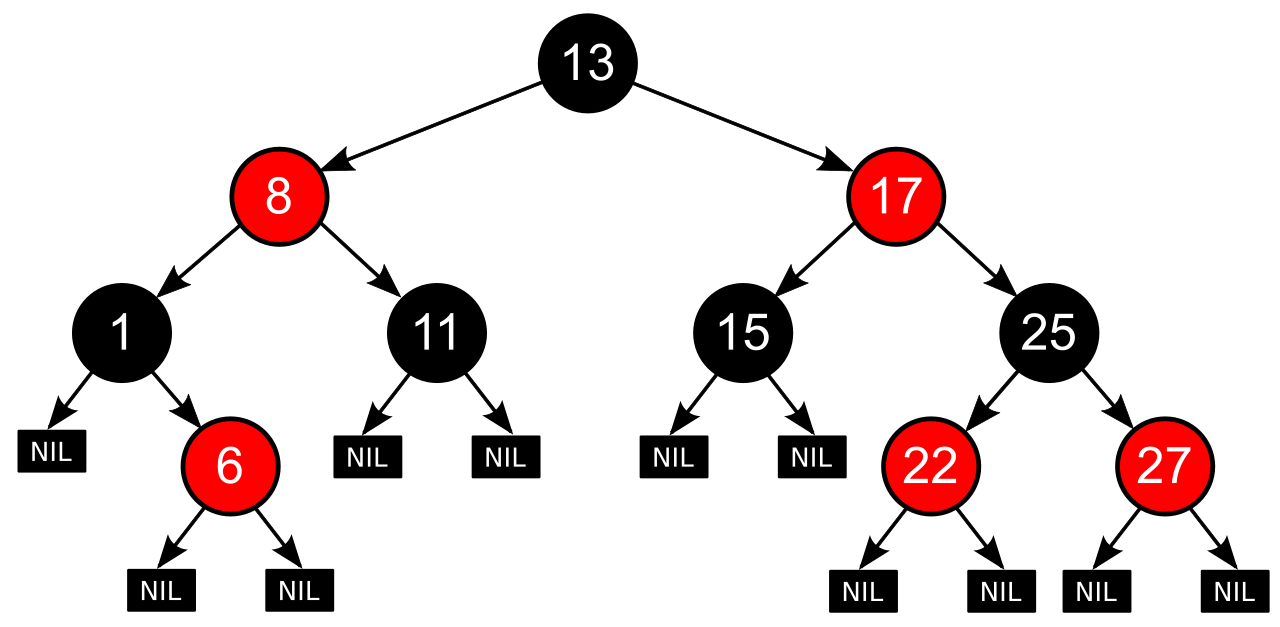
\includegraphics[width=\textwidth]{img/rbtree.png}
\end{columns}
\end{frame}


\begin{frame}{Contents}
  \setbeamertemplate{section in toc}[sections numbered]

  \tableofcontents%[hideallsubsections]
\end{frame}

\section{Verifying a Red-Black Tree}

\begin{frame}{Red-Black Tree}
\begin{columns}[T]
\column{0.5\textwidth}
\begin{itemize}
  \item Binary search tree
  \only<2->{
    \item Lookup, insertion and deletion in $\mathcal{O}(\log n)$ time
    \item But only if well balanced
  }
  \only<3->{
    \item Red-Black Tree uses colouring to automatically rebalance at insertion
    and deletion
  }
\end{itemize}

\column{0.5\textwidth}
\centering
\only<1>{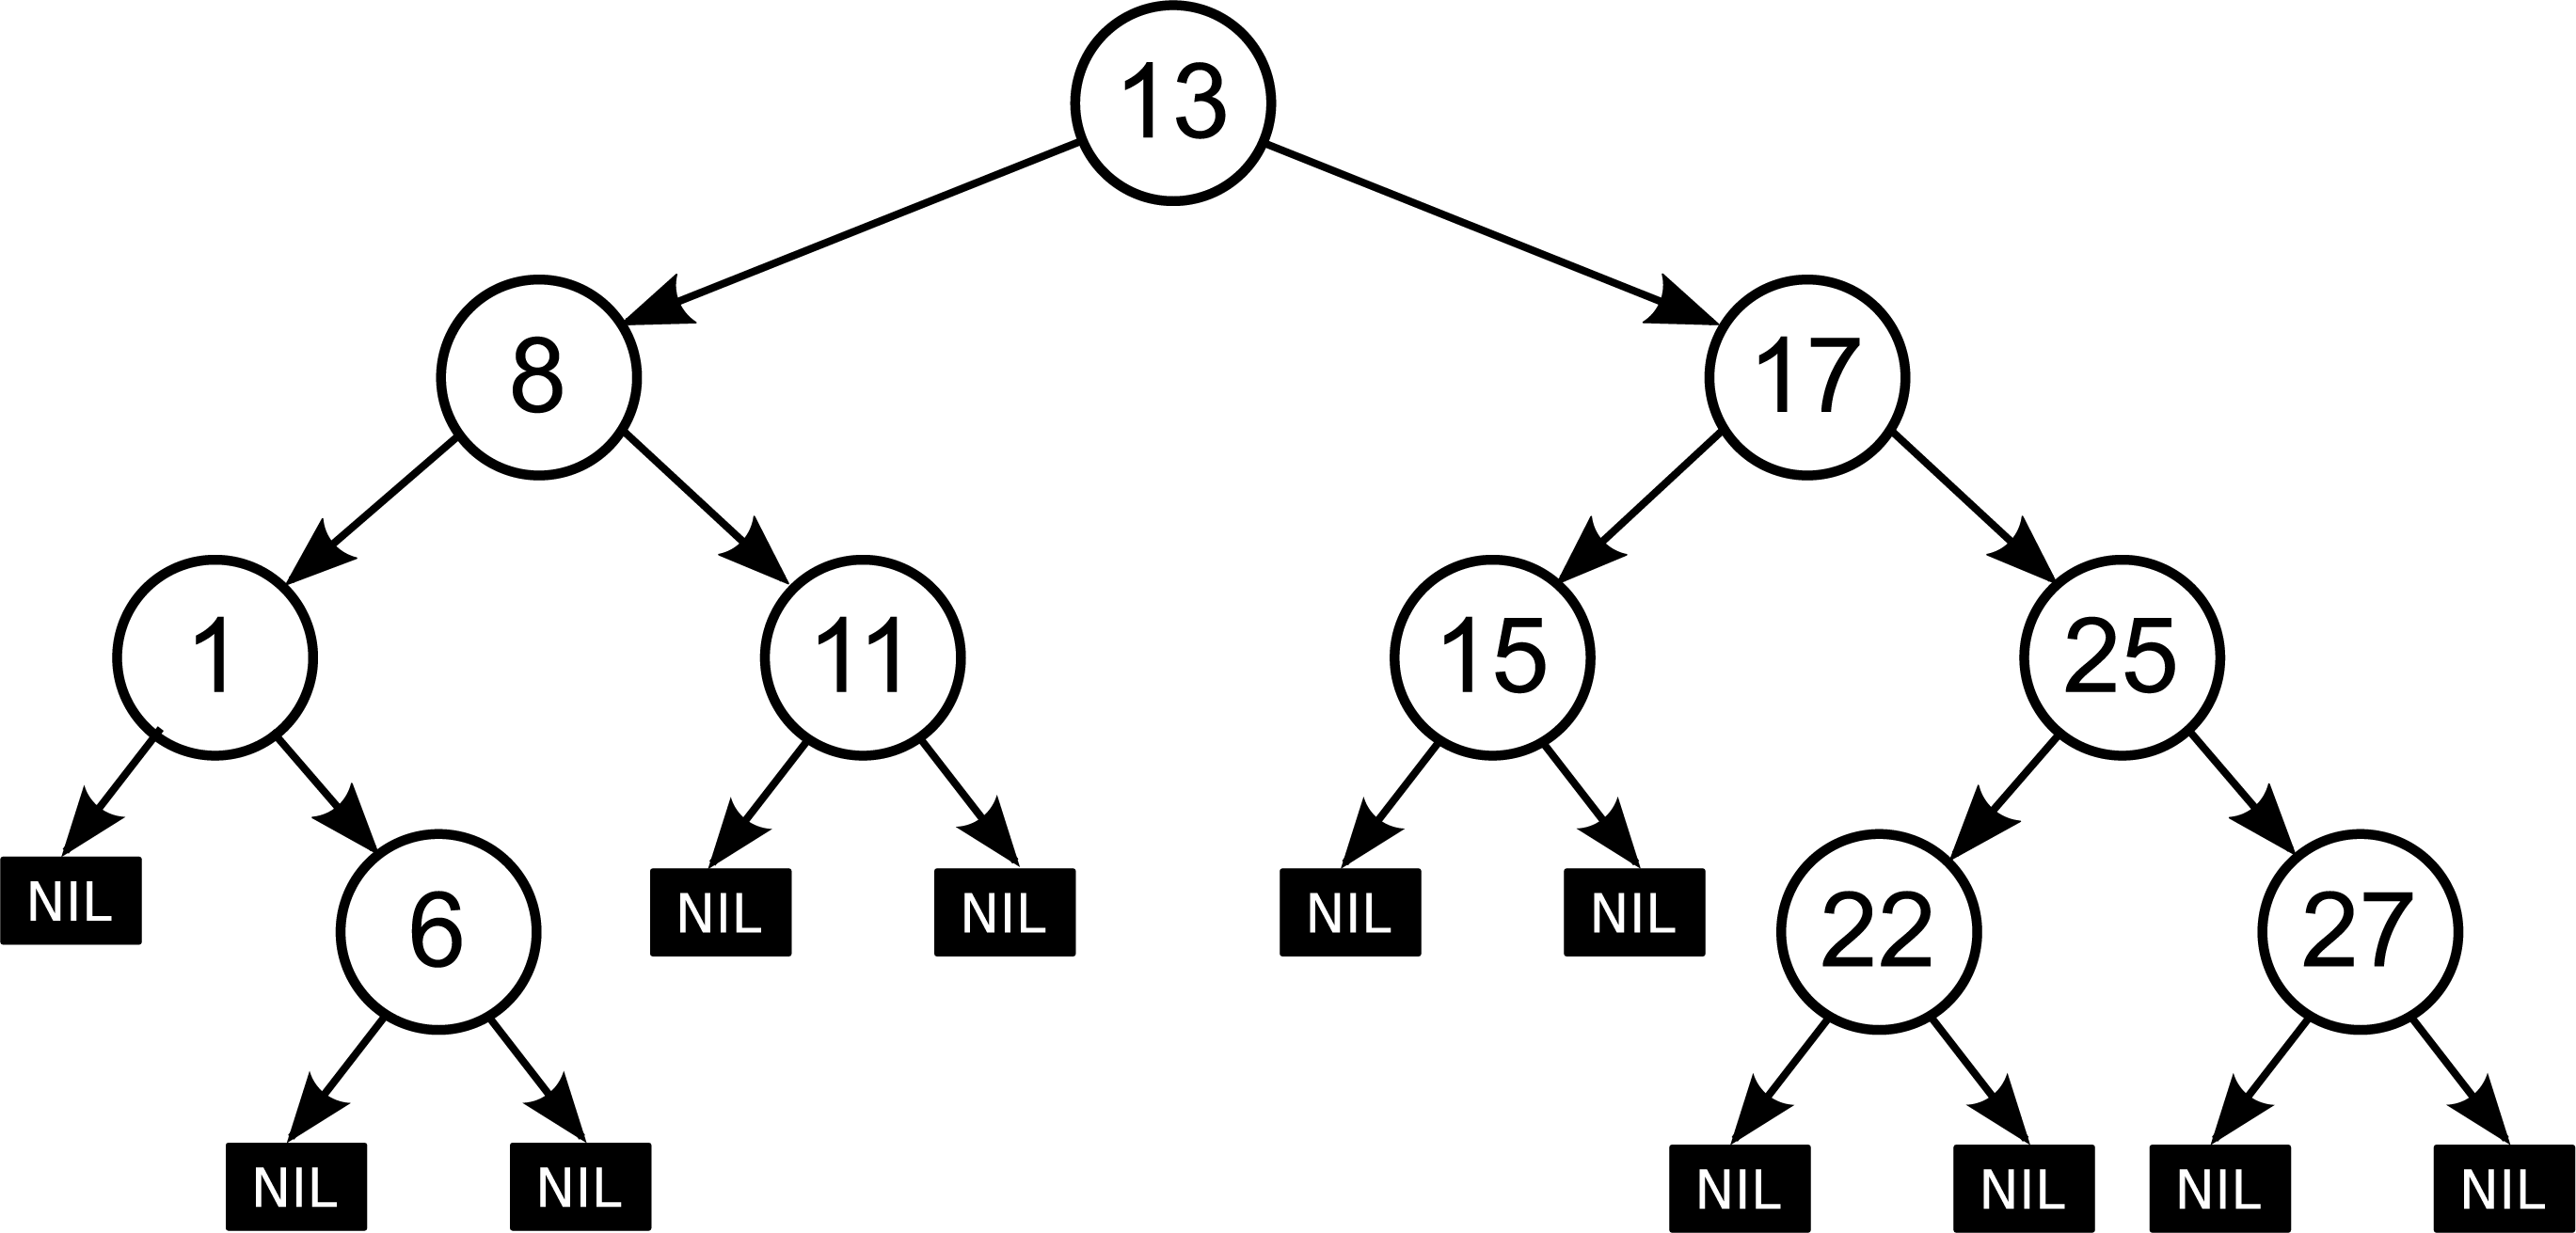
\includegraphics[width=\textwidth]{img/binary_tree.png}}
\only<2>{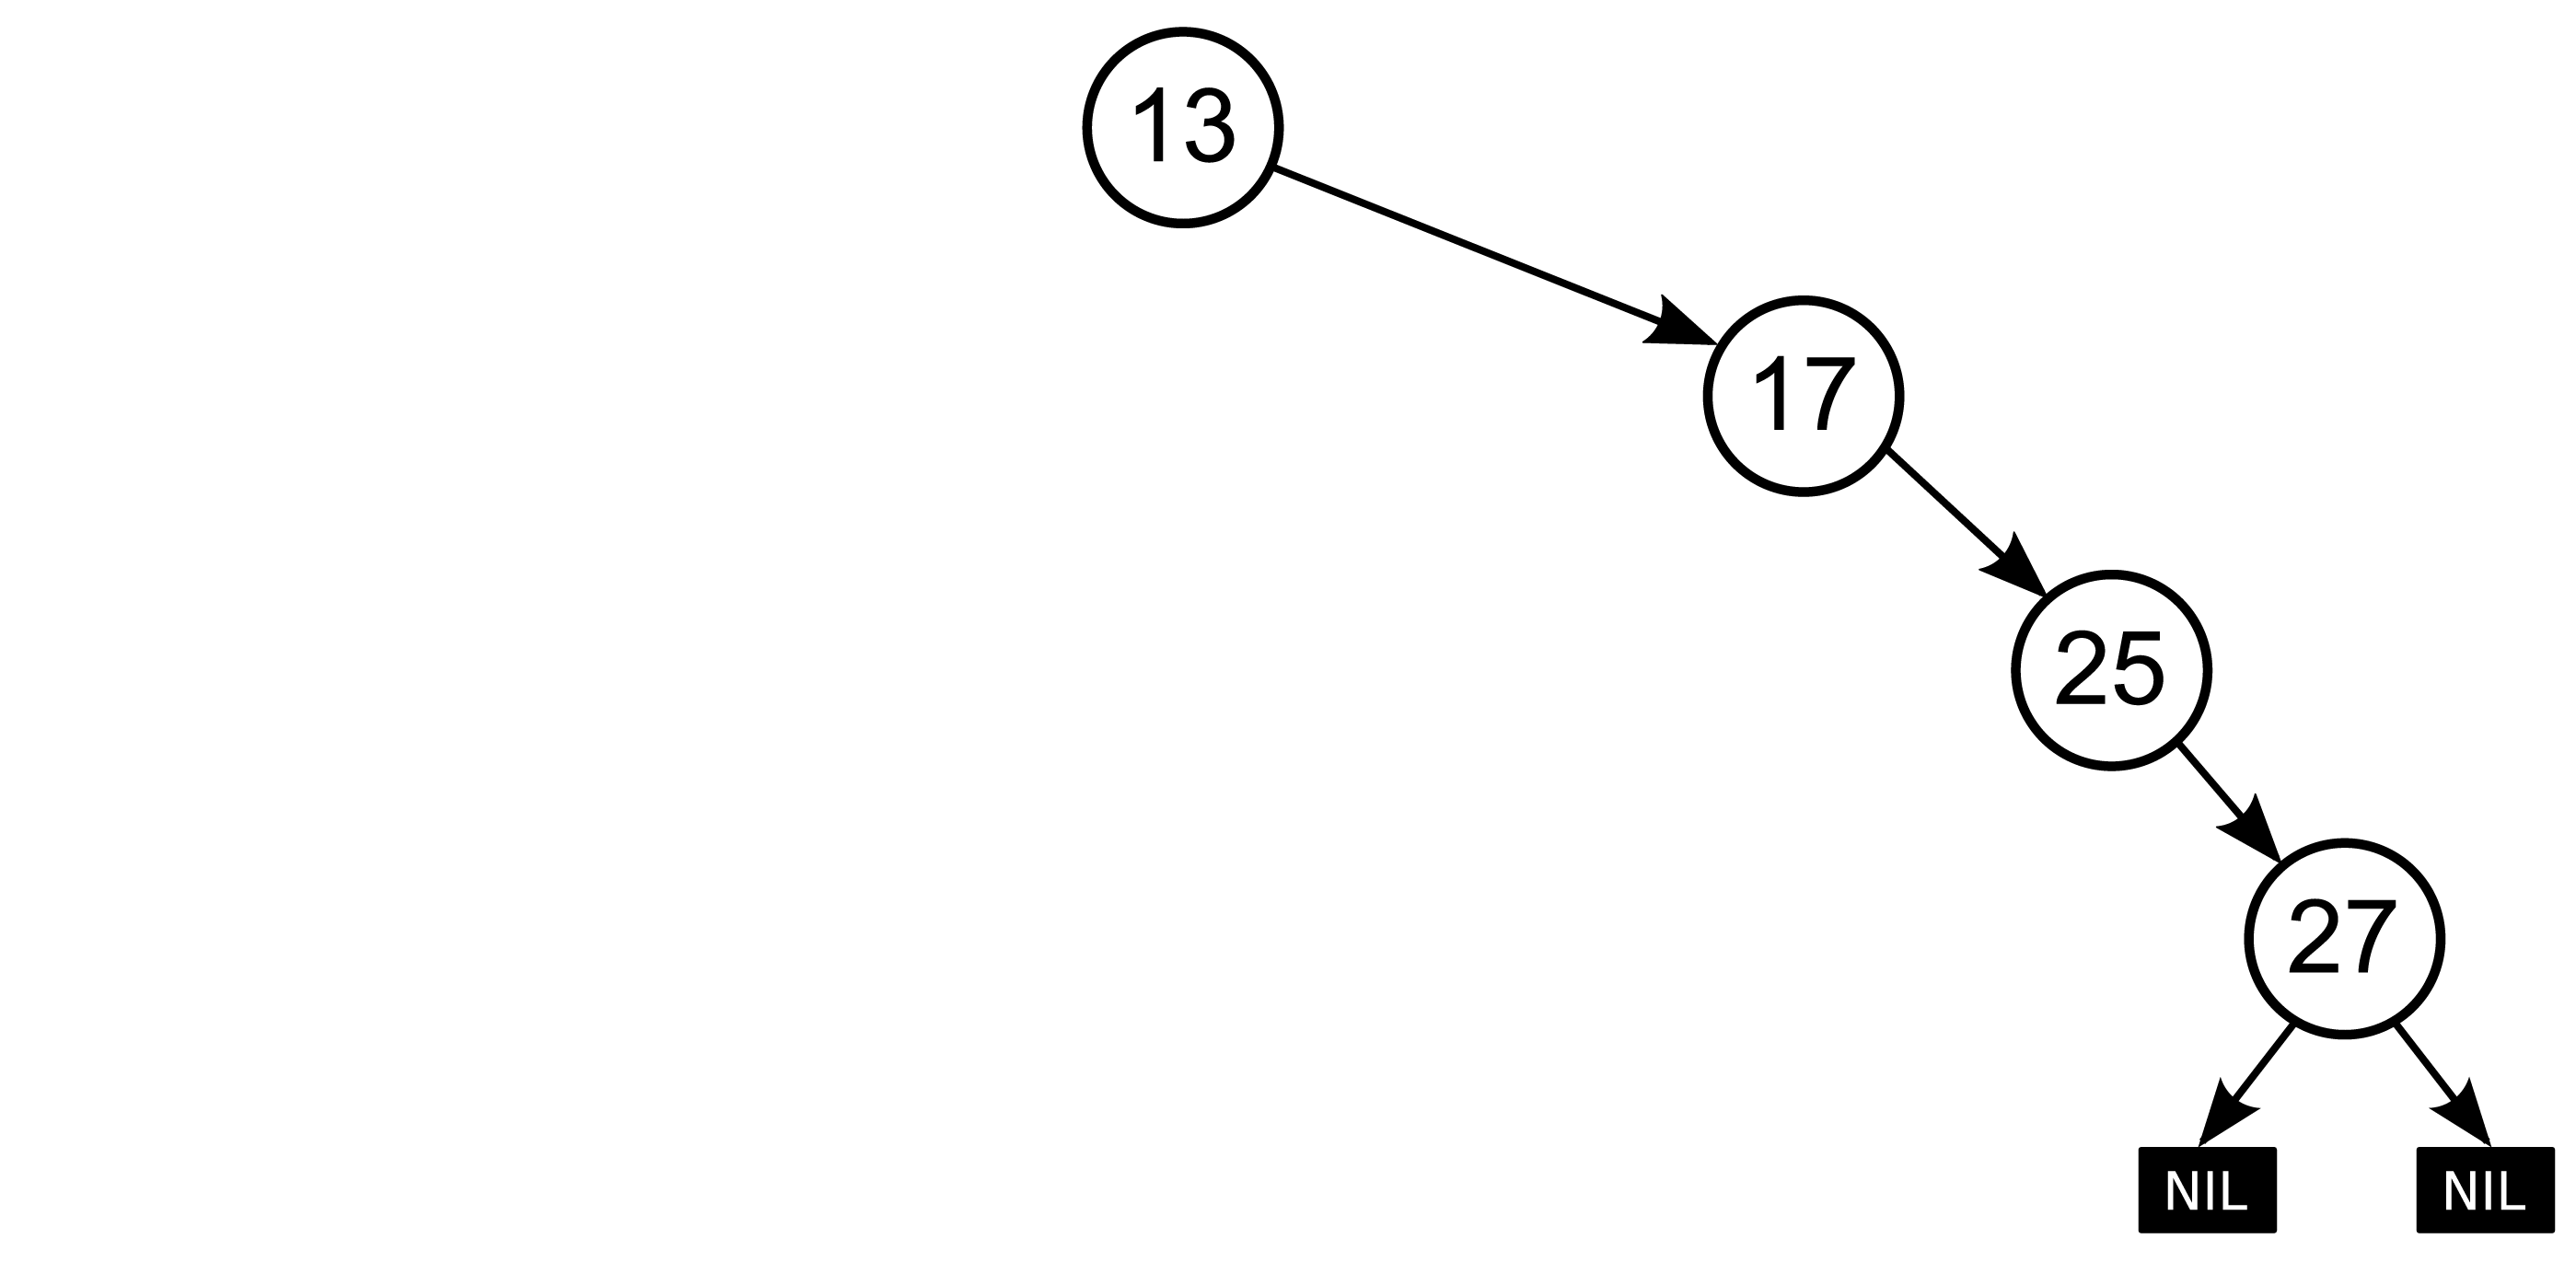
\includegraphics[width=\textwidth]{img/binary_tree_unbalanced.png}}
\only<3>{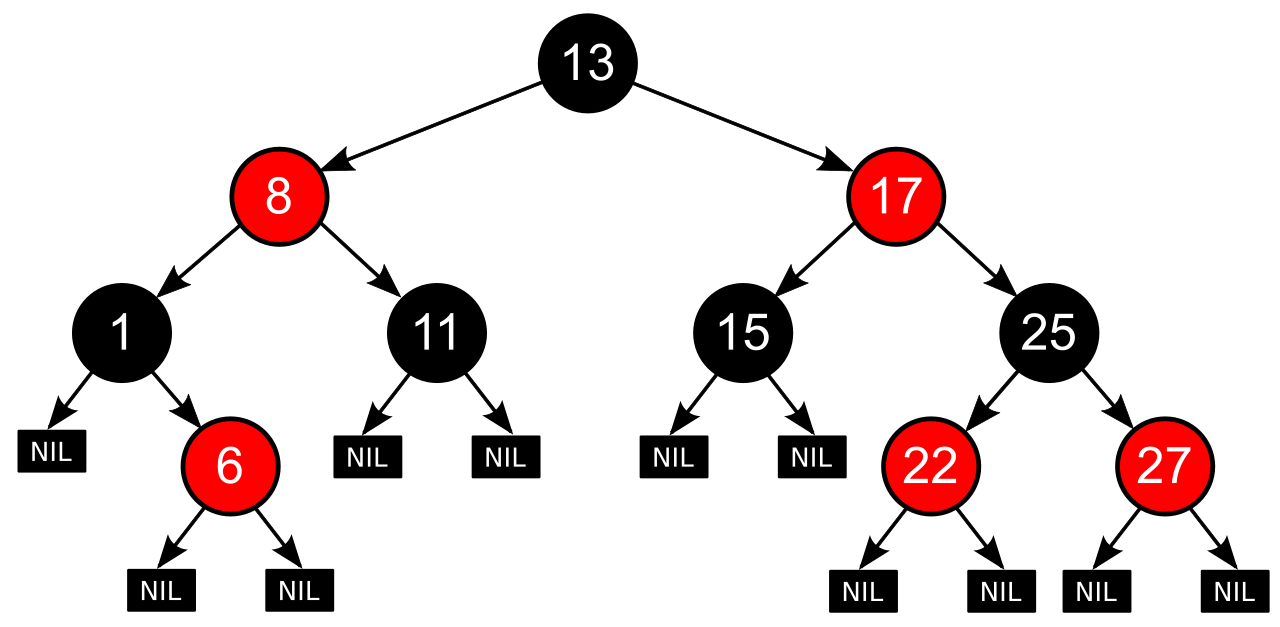
\includegraphics[width=\textwidth]{img/rbtree.png}}
\end{columns}
\end{frame}

\begin{frame}[standout]
  Why verify it?
\end{frame}

\begin{frame}{Red-Black Tree}
\textbf{Properties} \cite{rbtree}
\begin{columns}[T]
\column{0.5\textwidth}
\begin{enumerate}
  \item Each node is either red or black.
  \item All NIL (empty) nodes are considered black.
  \item A red node does not have a red child.
  \item Every path from a given node to any of its descendant NIL nodes goes through the same number of black nodes.
  \only<2>{\item The root is black.}
\end{enumerate}

\column{0.5\textwidth}
\centering
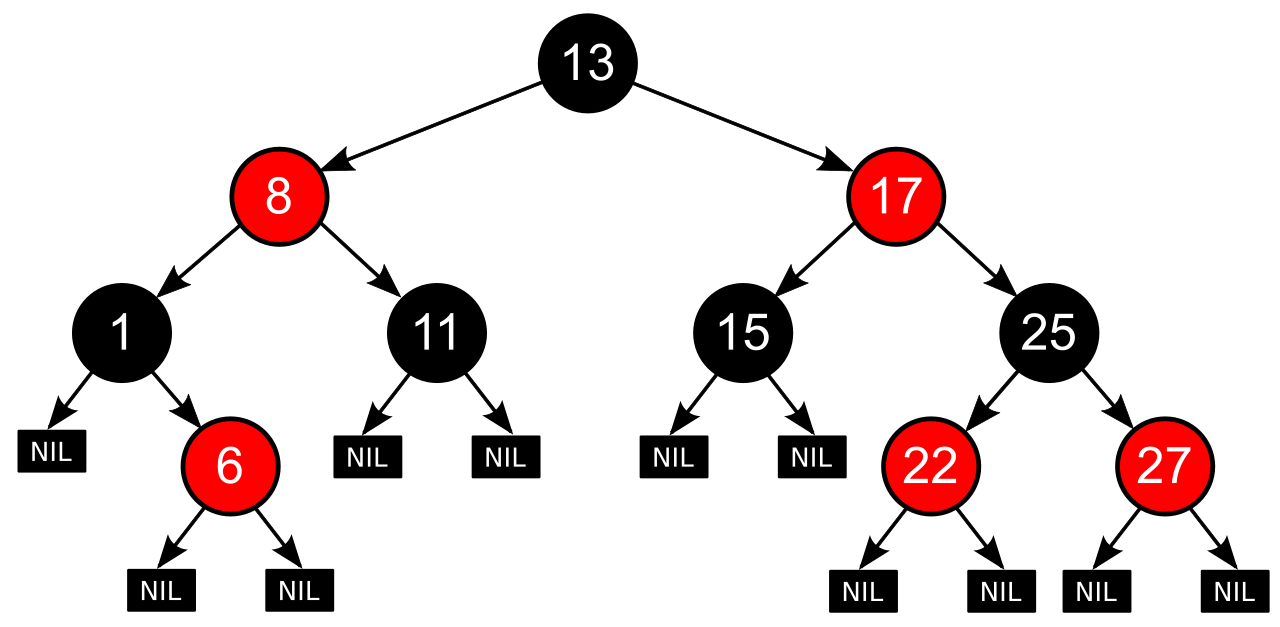
\includegraphics[width=\textwidth]{img/rbtree.png}
\end{columns}
\end{frame}

\begin{frame}{Insertion}
\begin{columns}[T]
\column{0.5\textwidth}
\textbf{Algorithm}
\begin{enumerate}
  \item Recursively descend in tree to correct position
  \only<2>{
    \item Insert a new red node
    \item Recursively go back up and solve all property violations
  }
\end{enumerate}

\column{0.5\textwidth}
\centering
\only<1>{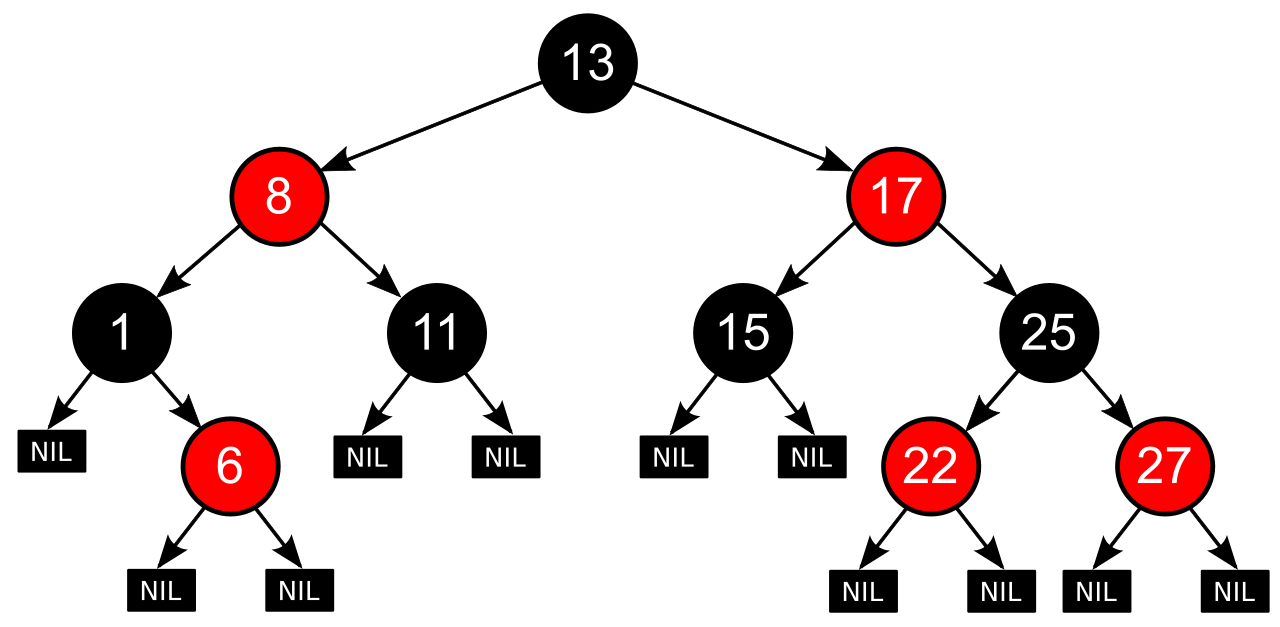
\includegraphics[width=\textwidth]{img/rbtree.png}}
\only<2>{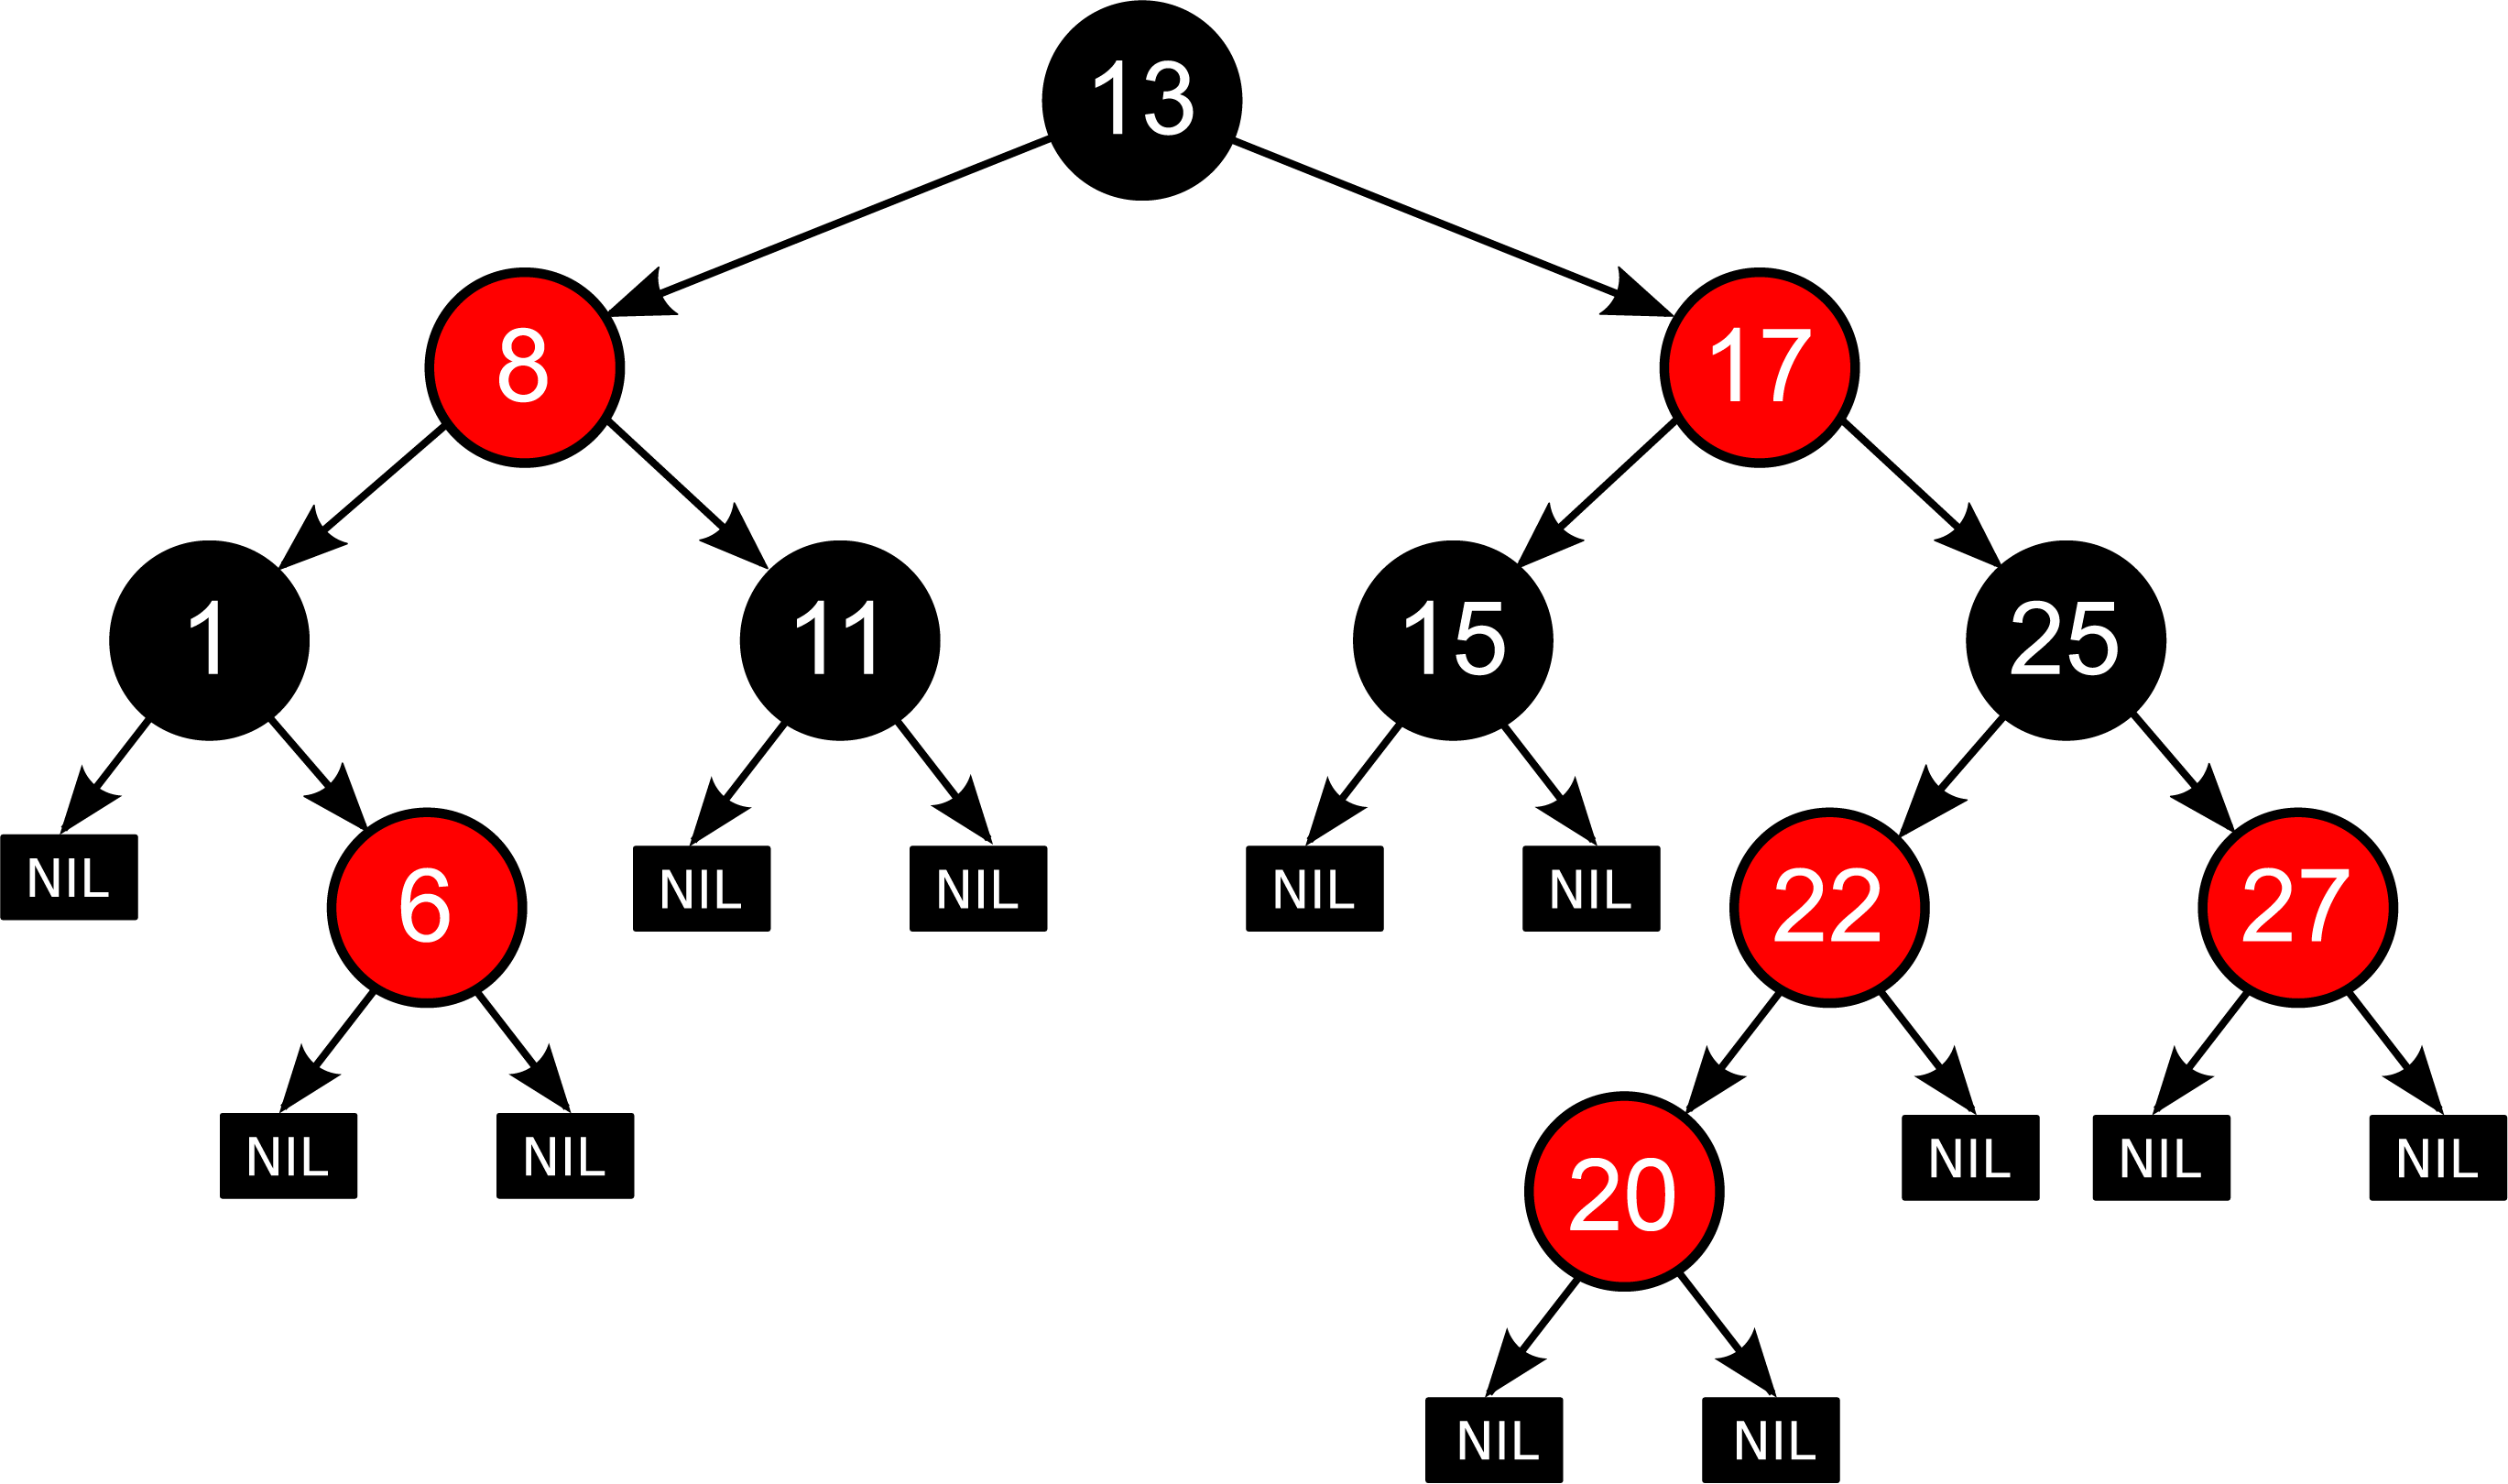
\includegraphics[width=\textwidth]{img/rbtree_insert.png}}
\end{columns}
\end{frame}

\begin{frame}[fragile]{Insertion}
In Scala
\begin{lstlisting}[language=Scala, basicstyle=\footnotesize\ttfamily,]
def ins(x: BigInt, t: Tree): Tree = {
  require(redNodesHaveBlackChildren(t) && blackBalanced(t))
  t match {
    case Empty() => Node(Red(),Empty(),x,Empty())
    case Node(c,a,y,b) =>
      if      (x < y)  balance(c, ins(x, a), y, b)
      else if (x == y) Node(c,a,y,b)
      else             balance(c,a,y,ins(x, b))
  }
} ensuring (res => content(res) == content(t) ++ Set(x)
                 && size(t) <= size(res) && size(res) <= size(t) + 1
                 && redDescHaveBlackChildren(res)
                 && blackBalanced(res))
\end{lstlisting}
\end{frame}

\begin{frame}{Rebalancing}
  \centering
  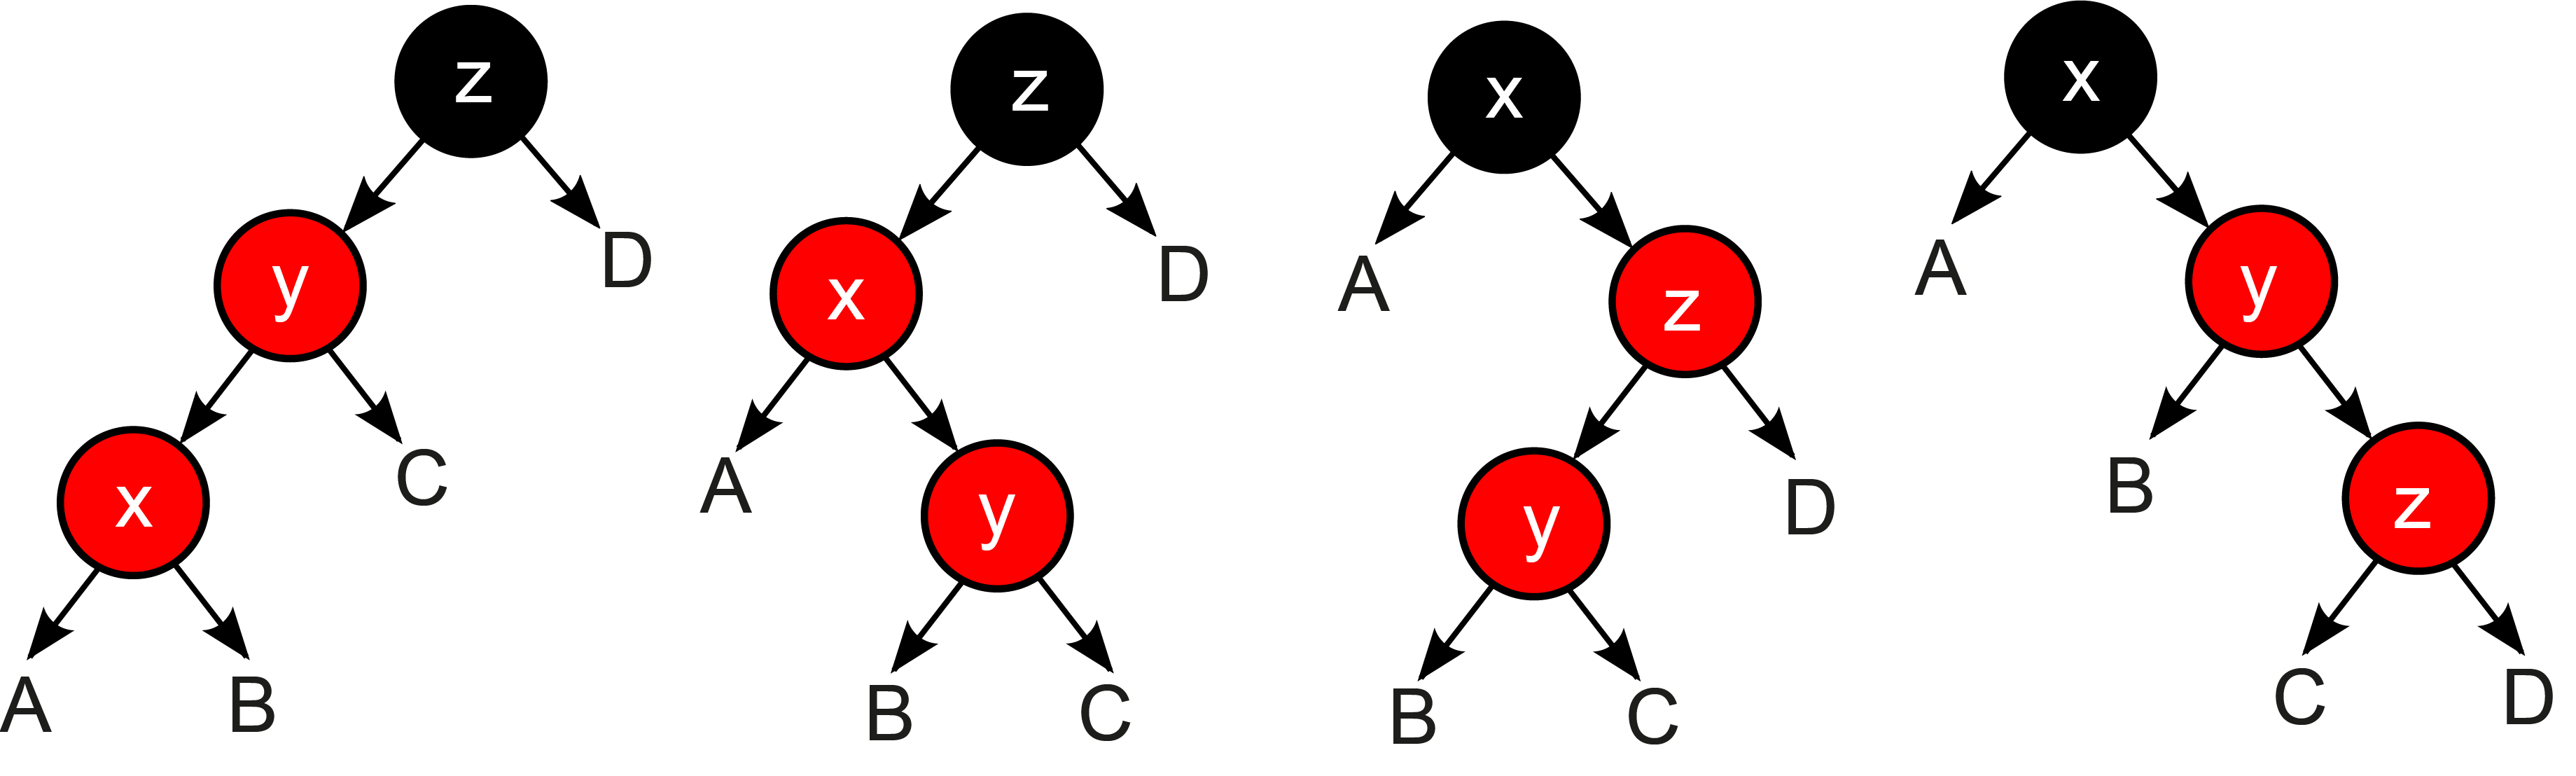
\includegraphics[width=0.8\textwidth]{img/rbtree_cases.png}
  \vfill
  \only<2>{
    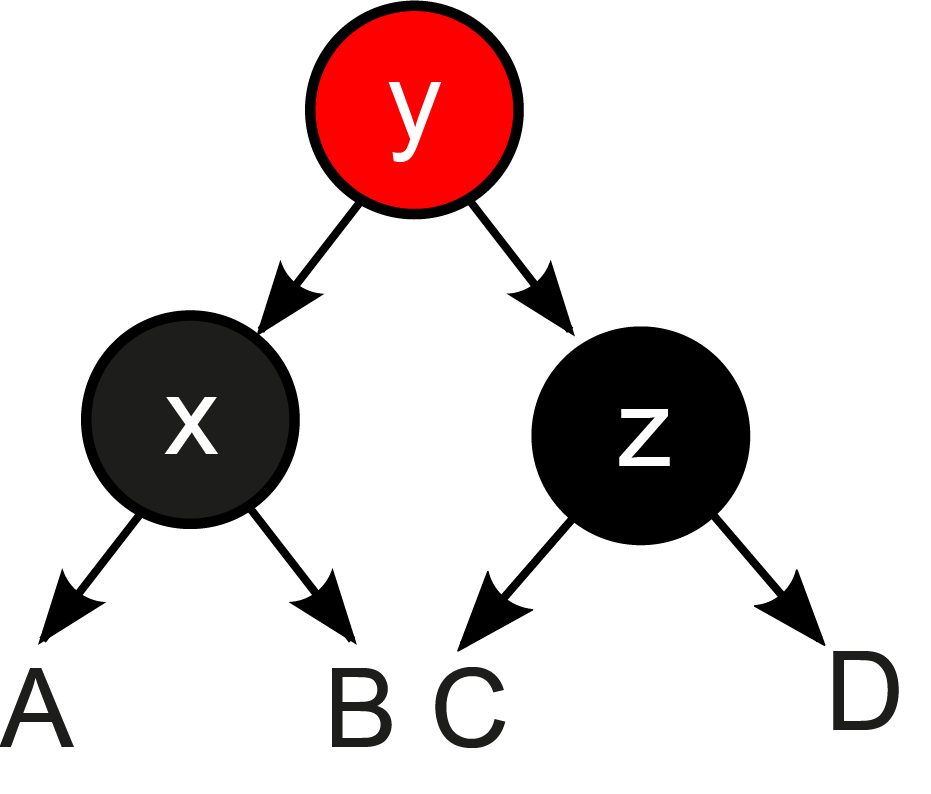
\includegraphics[width=0.3\textwidth]{img/rbtree_solution.png}
  }
\end{frame}

\begin{frame}[fragile]{Rebalancing}
In Scala
\begin{lstlisting}[language=Scala, basicstyle=\footnotesize\ttfamily,]
def balance(c: Color, a: Tree, x: BigInt, b: Tree): Tree = {
    Node(c,a,x,b) match {
      case Node(Black(),Node(Red(),Node(Red(),a,xV,b),yV,c),zV,d) =>
        Node(Red(),Node(Black(),a,xV,b),yV,Node(Black(),c,zV,d))
      case Node(Black(),Node(Red(),a,xV,Node(Red(),b,yV,c)),zV,d) =>
        Node(Red(),Node(Black(),a,xV,b),yV,Node(Black(),c,zV,d))
      case Node(Black(),a,xV,Node(Red(),Node(Red(),b,yV,c),zV,d)) =>
        Node(Red(),Node(Black(),a,xV,b),yV,Node(Black(),c,zV,d))
      case Node(Black(),a,xV,Node(Red(),b,yV,Node(Red(),c,zV,d))) =>
        Node(Red(),Node(Black(),a,xV,b),yV,Node(Black(),c,zV,d))
      case Node(c,a,xV,b) => Node(c,a,xV,b)
    }
  } ensuring (res => content(res) == content(Node(c,a,x,b)))
\end{lstlisting}
\end{frame}

\begin{frame}[standout]
  Why in Rust?
\end{frame}

\begin{frame}{Performance Comparison}
To insert the integers from 1 to 5000 into the implementation takes:
\begin{itemize}
  \item Red-Black Tree in Scala, fully functional, no mutation: 185s
  \only<2>{
    \item  Red-Black Tree in Rust, fully mutable, no allocation
    in rebalancing: \textbf{10ms}
  }
\end{itemize}
\end{frame}

\begin{frame}[fragile]{Red-Black Tree in Rust}
\begin{lstlisting}[language=Rust, caption={Data types with heap-allocation}]
enum Color {
  Red,
  Black,
}

enum RBTree<T> {
  Empty,
  Node(Color, Box<RBTree<T>>, T, Box<RBTree<T>>),
}
\end{lstlisting}
\end{frame}

\begin{frame}[fragile]{Red-Black Tree in Rust}
\begin{lstlisting}[language=Rust, caption={Insert method}]
impl RBTree<i32> {
  pub fn insert(&mut self, t: i32) {
    // Insert and color the root black.
    self.ins(t);
    if let Node(ref mut c, _, _, _) = self {
      *c = Black;
    }
  }
}
\end{lstlisting}
\end{frame}

\begin{frame}[fragile]{Red-Black Tree in Rust}
\begin{lstlisting}[language=Rust, caption={Insert method with specification}]
#[pre(
  self.red_nodes_have_black_children()
  && self.black_balanced()
)]
#[post(set_equals(
    &self.content(),&old(&self).content().insert(&t)
  ) && (old(&self).size() == self.size()
    || old(&self).size() + 1 == self.size())
  && self.red_nodes_have_black_children()
  && self.black_balanced()
)]
pub fn insert(&mut self, t: i32) { ... }
\end{lstlisting}
\end{frame}

\begin{frame}[fragile]{Red-Black Tree in Rust}
\begin{lstlisting}[language=Rust, caption={Recursive insertion}]
fn ins(&mut self, t: i32) {
  match self {
    Empty => {
      *self = Node(Red, Box::new(Empty), t, Box::new(Empty));
    }
    Node(_, left, value, right) => {
      if t < *value {
        left.ins(t); self.balance();
      } else if t > *value {
        right.ins(t); self.balance();
      }
    }
  }
}
\end{lstlisting}
\end{frame}

\begin{frame}[fragile]{Red-Black Tree in Rust}
\begin{columns}
\column{0.7\textwidth}
\begin{lstlisting}[language=Rust, caption={Balance imperatively}, basicstyle=\footnotesize\ttfamily,]
fn balance(&mut self) {
  match self {
    Node(Black, left, _, _) if left.is_red() => {
      match &mut **left {
        Node(Red, ll, _, _) if ll.is_red() => {
          self.rotate_right();
          self.recolor();
        }
        Node(Red, _, _, lr) if lr.is_red() => { ... }
        _ => {}
      }
    }
    Node(Black, _, _, right) if right.is_red() =>
      { ... }
    _ => {}
  }
}
\end{lstlisting}
\column{0.3\textwidth}
\centering
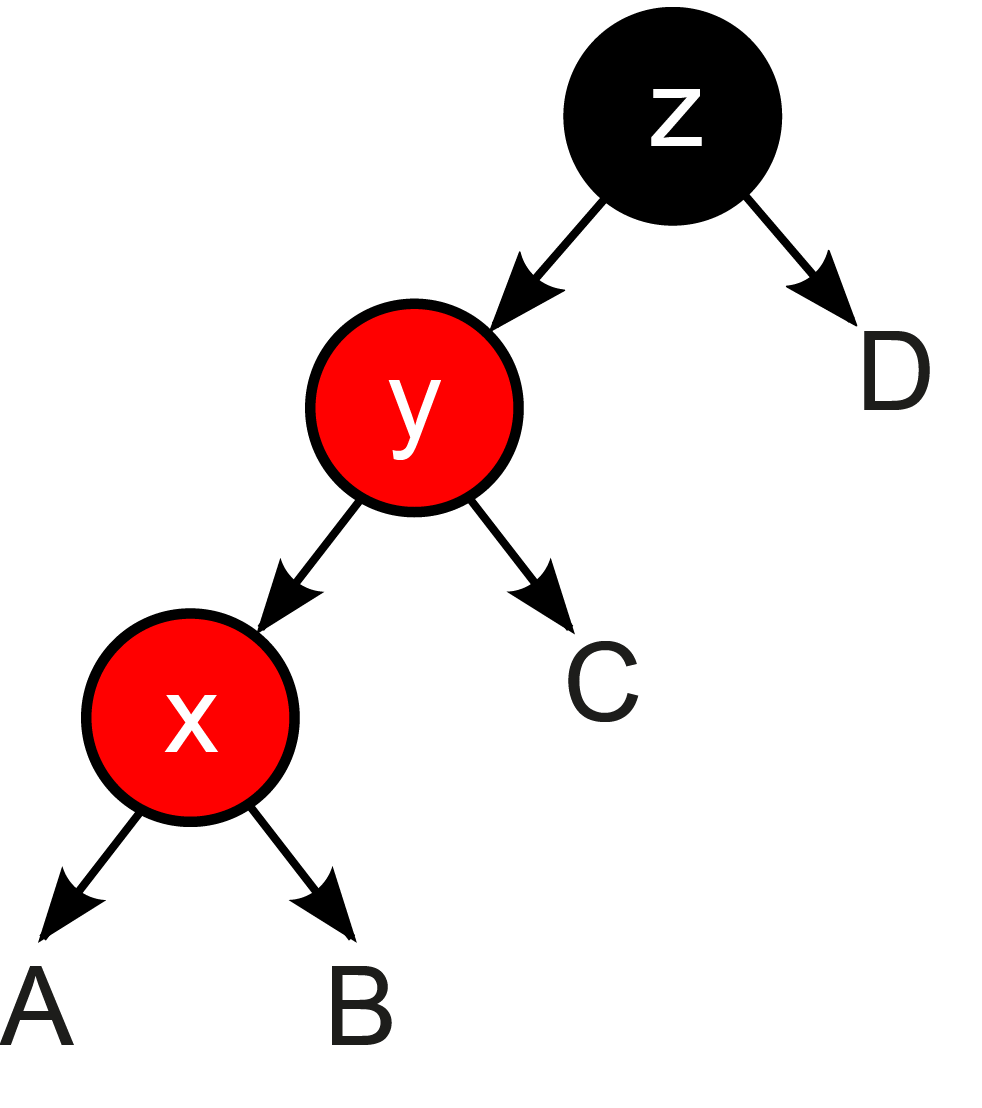
\includegraphics[width=0.8\textwidth]{img/rbtree_case_1.png}
\vspace{1cm}
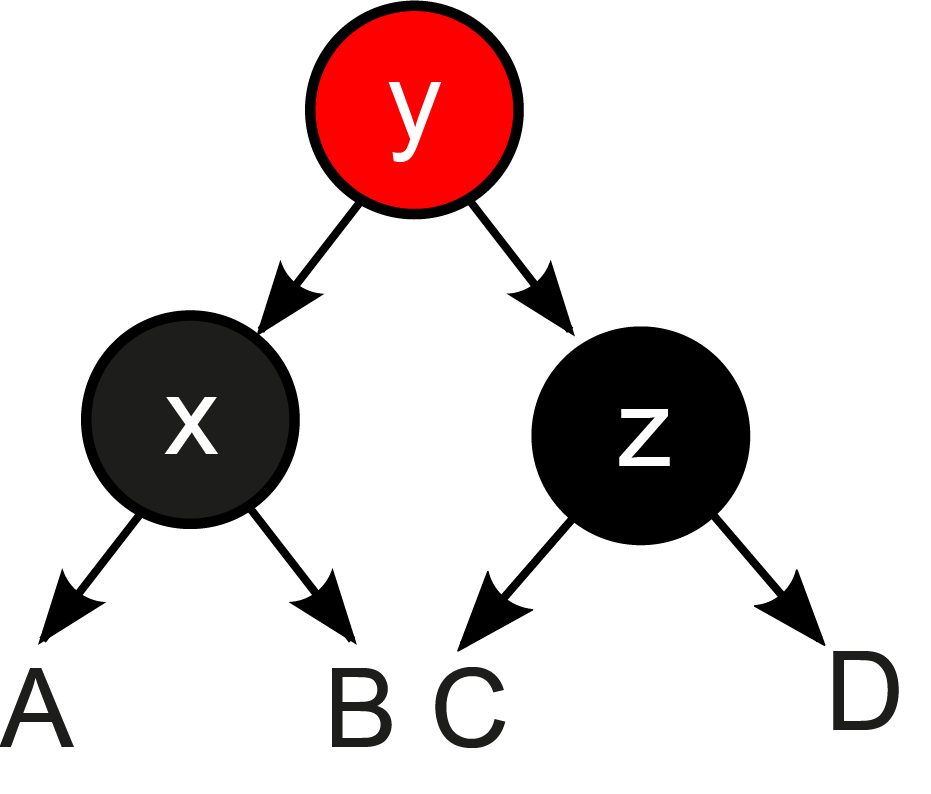
\includegraphics[width=0.8\textwidth]{img/rbtree_solution.png}
\end{columns}
\end{frame}


\begin{frame}[fragile]{Red-Black Tree in Rust}
\begin{columns}
\column{0.7\textwidth}
\begin{lstlisting}[language=Rust, caption={Tree rotation without allocation}, basicstyle=\footnotesize\ttfamily]
fn rotate_right(&mut self) {
  let self_tree = std::mem::replace(self, Empty);
  if let Node(c1, mut left, y, c) = self_tree {
    let left_tree = std::mem::replace(&mut *left, Empty);
    if let Node(c2, a, x, b) = left_tree {
      *left = Node(c1, b, y, c);
      *self = Node(c2, a, x, left);
    } else {
      *left = left_tree;
      *self = Node(c1, left, y, c);
    }
  }
}
\end{lstlisting}
\column{0.3\textwidth}
\centering
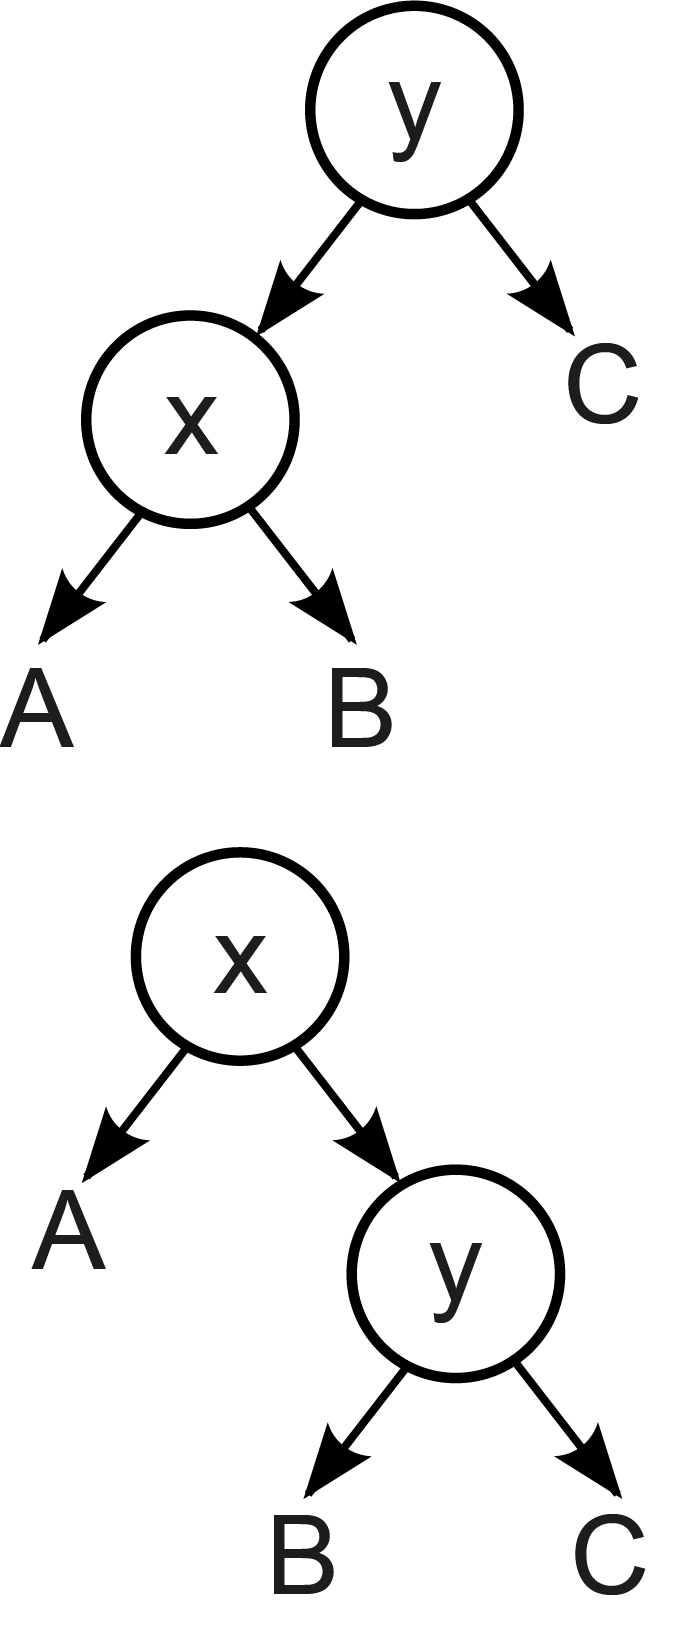
\includegraphics[width=0.6\textwidth]{img/rotate_right.png}
\end{columns}
\end{frame}


\begin{frame}{Spin it up}
\only<1>{
  OK, then let's try it!
  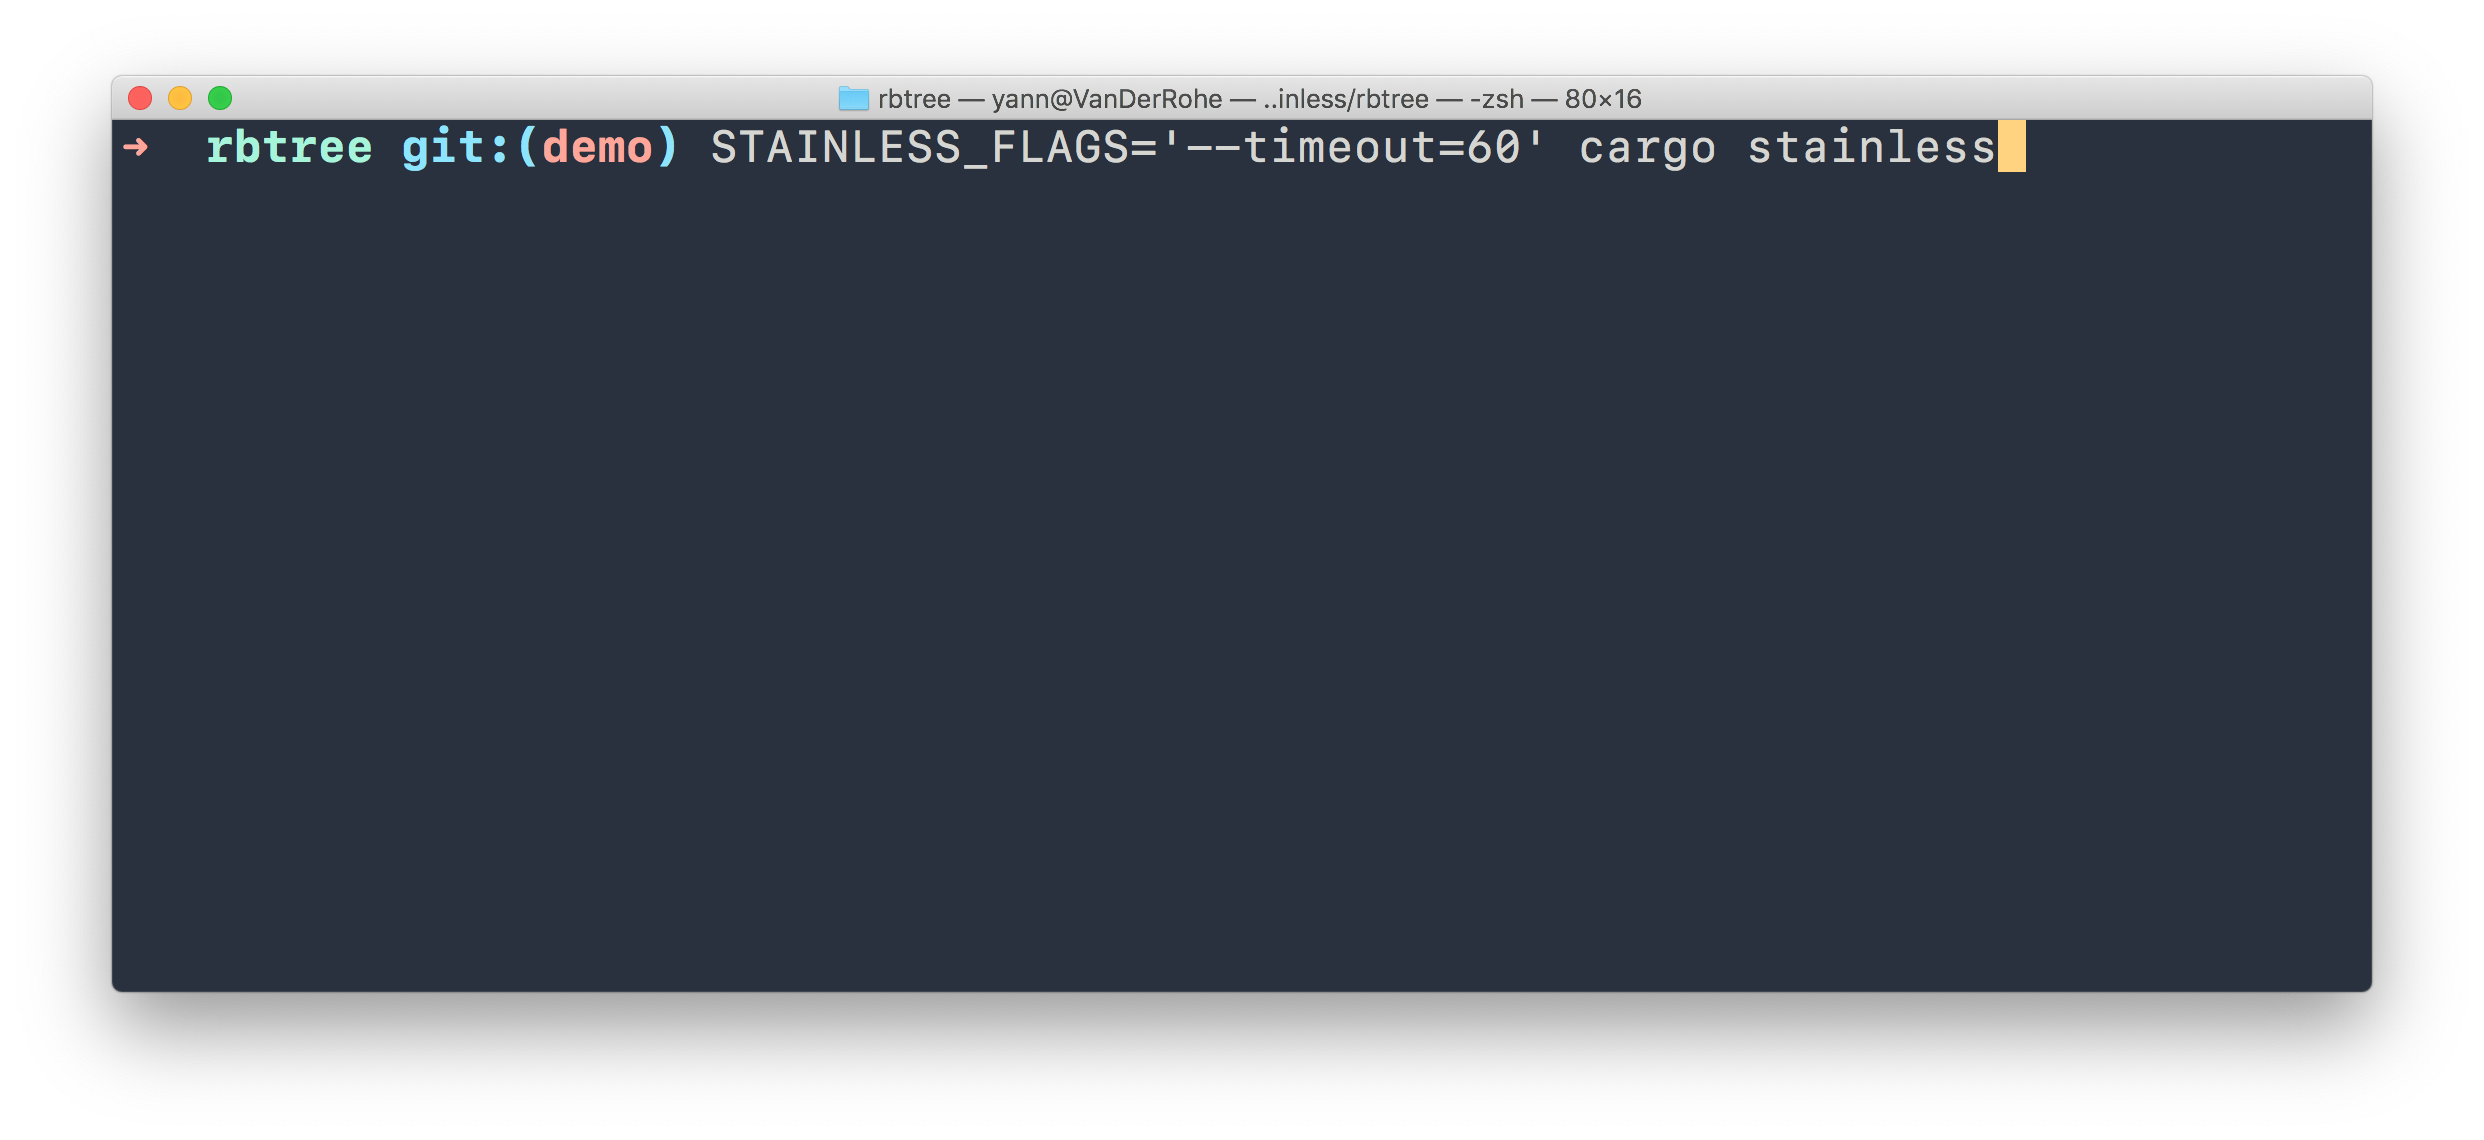
\includegraphics[width=\textwidth]{img/terminal_1.png}
}

\only<2>{
  \textbf{\alert{INVALID}} \\
  \texttt{
  - Result for 'postcondition' VC for balance @?:?:\\
  ...\\
    => INVALID\\
  Found counter-example:\\
    self: MutCell[RBTree[Int]] -> ...
  }
}
\end{frame}

\begin{frame}[fragile]{Red-Black Tree in Rust}
\begin{onlyenv}<1>
\begin{lstlisting}[language=Rust]
fn balance(&mut self) {
  match self {
    Node(Black, left, _, _) if left.is_red() => {
      match &mut **left {
        Node(Red, ll, _, _) if ll.is_red() => { ... }
        ...
      }
    }
    Node(Black, _, _, right) if right.is_red() => { ... }
    _ => {}
  }
}
\end{lstlisting}
\end{onlyenv}
\begin{onlyenv}<2>
\begin{lstlisting}[language=Rust, caption={Solved bug in balance function}]
fn balance(&mut self) {
  if let Node(Black, left, _, _) = self {
    if left.is_red() {
      match &mut **left {
        Node(Red, ll, _, _) if ll.is_red() => { ... }
        ...
      }
    }
  }
  if let Node(Black, _, _, right) = self {
    if right.is_red() { ... }
  }
}
\end{lstlisting}
\end{onlyenv}
\end{frame}

\begin{frame}{Required New Features}
\begin{itemize}
\item Heap-allocation
\item Methods on data types
\item Full support for mutability
\item Shared and mutable references
\item \lstinline!old! helper in postconditions
\end{itemize}
\end{frame}

\section{Tool Overview}

\section{Translation}

\subsection{Mutability}

\subsection{Traits to Type Classes}

\section{Conclusions}


\begin{frame}[allowframebreaks]{References}
  \bibliography{bib}
  \bibliographystyle{IEEEtranS}
\end{frame}


\appendix
